\documentclass[11pt]{beamer}
\usetheme{metropolis}  
\usecolortheme{dove}
\usepackage{hyperref}
\usepackage{bigints}
\usepackage{amsmath}
\usepackage{multicol}
\title{T\'opicos de investigaci\'on  CM072}
 \usepackage[spanish]{babel}
 \decimalpoint
\date{\today}
\author{C\'esar Lara Avila}
\institute{\url{https://github.com/C-Lara}}
\begin{document}
  \maketitle
  \section{1. Introducci\'on al Machine Learning }
  
\begin{frame}{Acerca del curso:}
	

\begin{itemize}
	\item \textcolor{violet}{P\'agina inicial al curso}
	\begin{itemize}
		\item \url{https://https://github.com/C-Lara/Curso-CM072}.
	\end{itemize}
	\item \textcolor{yellow}{Horarios:}
	\begin{itemize}
		\item Mi\'ercoles de 12-2pm Sala2. 
	\end{itemize}
\item \textcolor{blue}{Evaluaci\'on:} 
\begin{itemize}
	\item En el curso de tomaran  asignaciones por cada clase, las mejores asignaciones ser\'an las notas de las calificadas.
	\item Examen parcial y final en clase utilizando cuadernos de jupyter.
	\item Proyecto parcial y final del curso. 
	\item En la p\'agina web del curso se indica informaci\'on de las evaluaciones.
\end{itemize}
\end{itemize}
\end{frame}

\begin{frame}{Prerequisitos}
\textbf{Requerido:}

\begin{itemize}
\item \textcolor{orange}{Algoritmos b\'asicos}
\begin{itemize}
	\item An\'alisis de algoritmos, programaci\'on din\'amica.
	\item Nociones de an\'alisis de datos.
\end{itemize}
\end{itemize}

\textbf{Muy recomendado:}
\begin{itemize}
\item \textcolor{brown}{\'Algebra Lineal}
\begin{itemize}
	\item Matrices, vectores, sistema de ecuaciones lineales.
	\item Autovalores y autovectores, rango de una matriz.
	\item Valores singulares. Descomposiciones matriciales.
\end{itemize}
\item \textcolor{red}{C\'alculo multivariado}
\begin{itemize}
	\item Derivaci\'on, integraci\'on, plano tangente.
	\item Optimizaci\'on y multiplicadores de Lagrange.
\end{itemize}
\end{itemize}
\end{frame}

\begin{frame}{Libros y referencias}
El libro de referencia es el de David Barber, \href{http://web4.cs.ucl.ac.uk/staff/D.Barber/pmwiki/pmwiki.php?n=Brml.Online}{\textcolor{orange}{Bayesian Reasoning and Machine Learning}} de Cambridge University Press, 2017.

\vspace{0.3cm}

Otras posibilidades son:

\begin{itemize}
	\small{
	\item \href{http://www.cs.ubc.ca/\%7Emurphyk/MLbook/index.html}{\textcolor{yellow}{Machine Learning: a Probabilistic}} de Kevin Murphy (2012).
	\item \href{http://research.microsoft.com/en-us/um/people/cmbishop/prml/}{\textcolor{red}{Pattern Recognition and Machine}} de Chris Bishop  (2006). 
	\item  \textcolor{blue}{Machine Learning refined: Foundations, Algorithms, and Applications} 1st Edition Jeremy Watt, Reza Borhani y Aggelos K. Katsaggelos, 2016.
	\item \textcolor{violet}{Data Science From Scratch: First Principles with Python} de Joel Grus 2015.
	}

\end{itemize}
\end{frame}

\section{2.?`Qu\'e es Machine Learning? }

 \begin{frame}{\textbf{\textcolor{violet}{Clasificaci\'on: Desde datos a clases discretas}} }
 	


\vspace{0.2cm}

\textbf{Filtrado de Spam (Bayesiano)}

\scriptsize{Este filtro est\'a basado en el teorema de Bayes para determinar un correo electr\'onico como spam o no. De wikipedia
	
	
\[
\mathbb{P}(S|W) = \frac{\mathbb{P}(W|S)\cdot\mathbb{P}(S)}{\mathbb{P}(W|S)\cdot \mathbb{P}(S) + \mathbb{P}(W|H)\cdot \mathbb{P}(H) }
\]

donde:


\begin{itemize}
\item $\mathbb{P}(S|W)$ es la probabilidad de que un mensaje es spam, a sabiendas de que la palabra a buscar est\'a en el mensaje.
\item $\mathbb{P}(S)$ es la probabilidad general de que cualquier mensaje dado es spam.
\item $\mathbb{P}(W|S)$ es la probabilidad de que la palabra a buscar aparece en los mensajes de spam.
\item $\mathbb{P}(H)$es la probabilidad general de que cualquier mensaje dado no es spam.
\item  $\mathbb{P}(W|H)$ es la probabilidad de que la palabra a buscar  aparezca en los mensajes leg\'itimos.
\end{itemize}
}


\end{frame}


\begin{frame}{\textbf{\textcolor{violet}{Clasificaci\'on: Desde datos a clases discretas}} }
\vspace{0.2cm}
	
	\textbf{Reconocimiento facial}
	
\scriptsize{El reconocimiento facial es el proceso de identificaci\'on de una o varias personas en im\'agenes o v\'ideos mediante an\'alisis y comparaci\'on de patrones. Los algoritmos de reconocimiento facial normalmente extraen las caracter\'isticas faciales y las comparan con una base de datos para obtener la mejor coincidencia.

\vspace{0.3cm}

\tiny{Proceso de reconocimiento facial y un ejemplo de im\'agenes de entrenamiento para cada orientaci\'on}

\vspace{0.3cm}


 \begin{columns}
 	\begin{column}{0.4\textwidth}
 		\centering
 		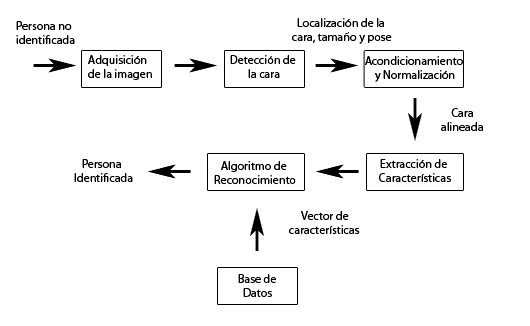
\includegraphics[width=1.3\textwidth]{ML2.png}
 	\end{column}
 	\begin{column}{0.3\textwidth}
 		\centering
 		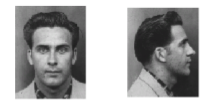
\includegraphics[width=0.6\textwidth]{ML0.png}
 	\end{column}
 	\begin{column}{0.25\textwidth}
 	\centering
 	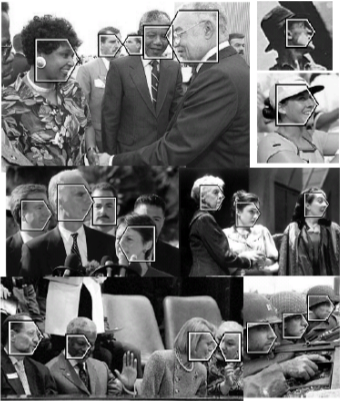
\includegraphics[width=1.1\textwidth]{ML1.png}	
 	\end{column}
 	​  \end{columns}
	
}
\end{frame}
\begin{frame}{\textbf{\textcolor{violet}{Clasificaci\'on: Desde datos a clases discretas}} }
	\vspace{0.2cm}
	
	\textbf{T\'ecnicas de reconocimiento facial}
	
	\scriptsize{ El reconocimiento facial aprovecha la visi\'on artificial para extraer informaci\'on discriminada de im\'agenes faciales y reconocimiento de patrones o t\'ecnicas del machine learning para modelar la apariencia de las caras y para clasificarlas. Por ejemplo:
		
	
		
	\begin{itemize}
		\item SVM
		\item \'Arboles de decisi\'on.
		\item M\'etodos de ensamblado.
		\item Redes neuronales profundas.
	\end{itemize}
	
De wikipedia:

El reconocimiento facial tridimensional, utiliza im\'agenes $3D$ tanto en el entrenamiento como en el reconocimiento. Esta t\'ecnica utiliza sensores en $3D$ para captar informaci\'on sobre la forma de la cara. Se utiliza un derivado del $PCA$ parcial, llamado, \textcolor{orange}{partial principal components analysis}.
}

\end{frame}

\begin{frame}{\textbf{\textcolor{violet}{Clasificaci\'on: Desde datos a clases discretas}} }
	\vspace{0.2cm}
	
	\textbf{Predicci\'on del tiempo}
	
	\scriptsize{No existen solamente procedimiento que recurren  \'unicamente a los modelos meteorol\'ogicos y climatol\'ogicos desarrollados para predecir el tiempo.
		
	\centering
	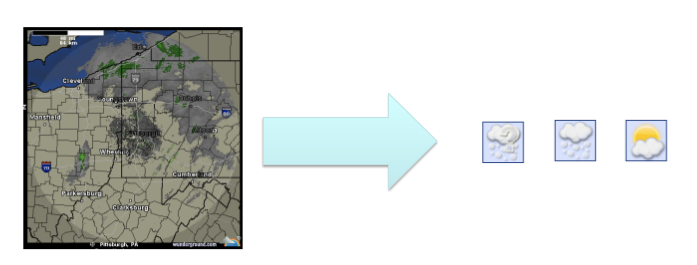
\includegraphics[width=0.8\textwidth]{ML3.png}	
	
 T\'ecnicas del machine learning, incluyendo modelos f\'isicos y redes neuronales profundas  empleando datos  hist\'oricos de las distintas variables meteorol\'ogicas (presi\'on atmosf\'erica, temperatura, punto de roc\'io, campo de vientos, etc) y de situaciones meteorol\'ogicas anteriores, para con los datos recabados en el momento presente, realizar previsiones con una buena precisi\'on .
	}
\end{frame}
\begin{frame}{\textbf{\textcolor{blue}{Regresi\'on que predice un valor num\'erico}}}
\vspace{0.2cm}
	
\textbf{Bolsa de valores}
	
\scriptsize{Una de las formas tanto en condiciones adversas, como en momentos normales en el mercado de predecir hacia donde ir\'a la bolsa as\'i como cada uno de sus valores se llama \texttt{\textcolor{violet}{an\'alisis t\'ecnico}}.

\vspace{0.3cm}

\centering
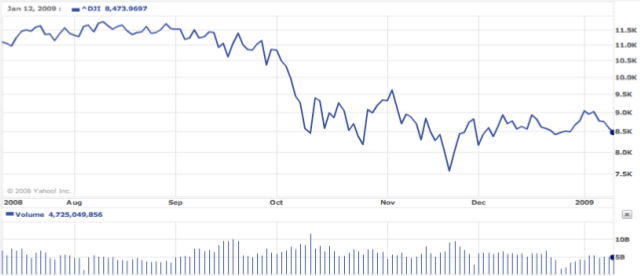
\includegraphics[width=0.65\textwidth]{ML4.png}	

\vspace{0.3cm}
	
El an\'alisis t\'ecnico es un  estudio  de indicadores que se  presentan de forma gr\'afica informaci\'on b\'asica muy necesaria con el objetivo final de tomar una decisi\'on a corto plazo de compra o venta en esas acciones.}
\end{frame}

\begin{frame}{\textbf{\textcolor{blue}{Regresi\'on que predice un valor num\'erico}}}
	\vspace{0.2cm}

\textbf{An\'alisis t\'ecnico y regresi\'on}

\scriptsize{Principalmente el an\'alisis t\'ecnico se basa en un conjunto de operaciones estad\'isticas y matem\'aticas con los precios que van resultando en el mercado, para determinar y detectar situaciones en las tendencias que siguen las cotizaciones de esas acciones a corto y mediano plazo.
	
\begin{itemize}
	\item Econometr\'ia
	\item Matem\'atica financiera avanzada.
\end{itemize}	

El mercado se comporta de una manera gr\'afica tal que el an\'alisis t\'ecnico se puede comparar con un conjunto modelo de variables en las que intentamos predecir el comportamiento futuro con una recta de regresi\'on del tipo simple: $Y= a + bX$.

Es una forma muy b\'asica de predicci\'on, pero es la m\'as cercana a una explicaci\'on matem\'atica simple de c\'omo se realizan las predicciones de los futuros valores burs\'atiles.
}
	
\end{frame}

\begin{frame}{\textbf{\textcolor{blue}{Regresi\'on que predice un valor num\'erico}}}
	\vspace{0.2cm}
	
	\textbf{Predicci\'on del tiempo}
	
\scriptsize{La predicci\'on meteorol\'ogica ha sido tradicionalmente realizada por modelos f\'isicos de la atm\'osfera, que son inestables a las perturbaciones, y por lo tanto son imprecisos para grandes per\'iodos de tiempo. Las t\'ecnicas del machine learning son m\'as robustas a las perturbaciones,  por lo que  generan potencialmente pron\'osticos meteorol\'ogicos m\'as precisos durante grandes per\'iodos de tiempo.
	
\vspace{0.3cm}

\centering
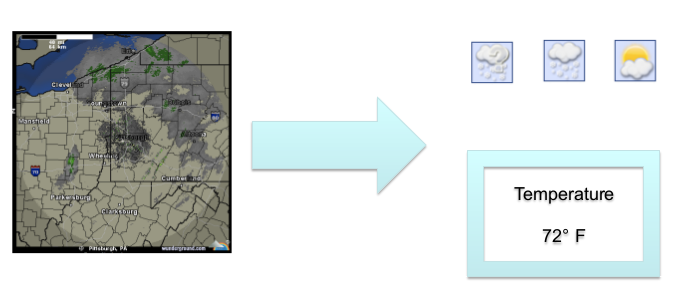
\includegraphics[width=0.7\textwidth]{ML5.png}	

En este contexto, podremos encontrar el valor de la temperatura en determinado escenario, utilizando regresi\'on lineal.}
\end{frame}


\begin{frame}{\textbf{\textcolor{red}{Filtrado colaborativo y basado en contenido}}}
\textbf{Recomendadores y tipos de filtros}

\vspace{0.2cm}

\scriptsize{Un \textcolor{blue}{recomendador} es un sistema que selecciona un producto que, si se compra, maximiza el valor tanto para el comprador como para el vendedor en un determinado momento del tiempo. 
	
Los recomendadores habitualmente son de dos tipos: los \textcolor{orange}{filtros colaborativos} y los \textcolor{violet}{filtros  basados en contenido}. En este contexto, un filtro es el algoritmo matem\'atico que decide cu\'al es la recomendaci\'on \'optima basado en los datos que le entreguemos.

\begin{itemize}
	\item Los filtros colaborativos generalmente basan su l\'ogica en las caracter\'isticas del usuario. Los datos que se tienen del usuario se convierten en el centro de un filtro colaborativo. Ejemplo: \href{https://www.reddit.com/}{reddit}, \href{https://www.youtube.com}{youtube}  y \href{https://www.last.fm/}{Last.fm}.
	
	\item Los filtros basados en contenido tienen el producto como base de la predicci\'on, en lugar de tener al usuario. Es decir, utiliza las caracter\'isticas del art\'iculo para hacer las recomendaciones. Ejemplo: \href{http://www.imdb.com/}{IMDb} o \href{https://www.rottentomatoes.com/}{Rotten Tomatoes}.
\end{itemize}  }
\end{frame}

\begin{frame}{\textbf{\textcolor{red}{Filtrado colaborativo }}}

\textbf{Algoritmos}

\begin{itemize}
	\scriptsize{
	\item Algoritmos de filtrado colaborativo basados en memoria, o algoritmos de vecinos cercanos(Nearest Neighbour).
}
\scriptsize{
\item Algoritmos de filtrado colaborativo basados en Modelo. Clustering o redes neuronales como las Redes de Funciones de Base Radial (RBFN).}
\end{itemize}

\vspace{0.2cm}

\scriptsize{Un sistema de recomendaciones es mucho m\'as que un algoritmo o un filtro que selecciona productos con m\'as o menos acierto. Podemos dividir un recomendador en $4$ partes: }

\begin{itemize}
	\item La base de conocimiento (la informaci\'on, los datos).
	\item El procesamiento de la base de conocimientos (tecnolog\'ia, algoritmos, filtros).
	\item Anal\'itica y control de negocio (medir todo, estrategia de negocio).
	\item Interface del usuario.
\end{itemize}	
	
\end{frame}


\begin{frame}{\textbf{\textcolor{violet}{Aprendizaje supervisado: Encuentra $f$}}}
	
\begin{itemize}
	\item \textbf{\textcolor{blue}{Dado:}} Un conjunto de entrenamiento $\{ x_i, y_i	\}|i = 1, \dots, N$
	\item \textbf{\textcolor{blue}{Encuentra:}} Una buena aproximaci\'on a $f: X \rightarrow Y$.
\end{itemize}

\vspace{0.3cm}

 \textbf{\textcolor{blue}{Ejemplos:}}
 
 \begin{itemize}
 	\item \textbf{\textcolor{blue}{Detecci\'on de spam:}}
 	\begin{itemize}
 		\item Mapea email a \{ Spam, no es Spam\}.
 	\end{itemize}
 	\item \textbf{\textcolor{blue}{Reconocimiento de d\'igitos}}
 	\begin{itemize}
 		\item  Mapea pixeles a $\{0,1, 2,3,4,5,6,7,8,9\}$.
 	\end{itemize}
 	\item \textbf{\textcolor{blue}{Predicci\'on de valores}}
 	\begin{itemize}
 		\item   Nuevas funciones, hist\'orico de precios, etc a $\mathbb{R}$ (los n\'umeros reales).
 	\end{itemize}
 \end{itemize}
\end{frame}

\begin{frame}{\textbf{\textcolor{green!55!blue}{Un problema de Aprendizaje supervisado}}}
\begin{columns}
	\begin{column}{0.5\textwidth}
	Conjunto de datos:
	
	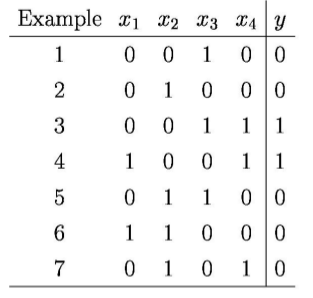
\includegraphics[scale= 0.45]{ML6.png}
	\end{column}
	\begin{column}{0.5\textwidth}  
	\begin{itemize}
		\item Nuestro prop\'osito es encontrar una funci\'on $f: X \rightarrow Y$
		\begin{itemize}
		\item $X = \{0,1\}^4$
		\item $Y = \{0, 1\}$
		\end{itemize}
	\item \textbf{\textcolor{blue}{Pregunta 1}} ?`C\'omo elegir el espacio de  hip\'otesis, el conjunto de funciones posibles $f$?
	\item \textbf{\textcolor{blue}{Pregunta 2}}?` C\'omo encontramos el mejor $f$ en el espacio de  hip\'otesis? 
	\end{itemize}
	\end{column}
\end{columns}
\end{frame}


\begin{frame}{\textbf{\textcolor{orange}{Crecimiento del Machine Learning}}}
\textbf{El machine learning es un enfoque de:}
\begin{itemize}
	\small{
	\item Reconocimiento de voz, Procesamiento del lenguaje natural.
	\item  Visi\'on por computador
	\item Control de robots
	\item Biolog\'ia computacional
	\item Redes de sensores
	\item \dots
}
\end{itemize}

\textbf{Esta tendencia se est\'a acelerando en:}
\small{
\begin{itemize}
	\item Big Data
	\item Algoritmos mejorados de Machine Learning
	\item Computadoras m\'as r\'apidas
	\item Buen software de c\'odigo abierto
	\item \dots
\end{itemize}
}
\end{frame}

\begin{frame}{\textbf{\textcolor{red}{Mapa del curso}}}
\textbf{Primera parte: Aprendizaje supervisado}

\begin{itemize}
	\item SVM, m\'etodos del Kernel.
	\item Teoria del aprendizaje.
	\item \'Arboles de decisi\'on, boosting, aprendizaje profundo.
\end{itemize}
\textbf{Segunda parte: Ciencia de datos}
\begin{itemize}
	\item Aprendizaje no supervisado. Algoritmo EM.
	\item Reducci\'on de la dimensi\'on.
\end{itemize}
\end{frame}

\begin{frame}{\textbf{\textcolor{green!55!blue}{Principio de la navaja de Ockham}}}

\begin{itemize}
\small{
\item  Guillermo de Ockham, fue un monje que vivi\'o en los a\~nos $1280-1349$.
\item Principio de parsimonia:}

\scriptsize{\texttt{No se debe aumentar, m\'as all\'a de lo necesario, el n\'umero de entidades necesarias para explicar cualquier cosa}}

\small{
\item Cuando hay \textcolor{red}{muchas} soluciones disponibles para un problema dado, debemos seleccionar la m\'as \textcolor{red}{simple}. Pero, ?`qu\'e entendemos por \textcolor{red}{simple}?

\item Usaremos el \textcolor{red}{conocimiento previo (prior)} del problema para resolver para definir lo que es
una soluci\'on simple.

\centering
\scriptsize{\texttt{Ejemplo de un prior: smoothness}}
}
\end{itemize}
\end{frame}

\begin{frame}{\textbf{\textcolor{blue}{Aspectos claves del Machine Learning}}}
	
\begin{itemize}
\small {
	\item  ?`C\'omo elegimos un espacio de hip\'otesis?}
	\begin{itemize}
	\scriptsize{
	\item Con frecuencia utilizamos el conocimiento previo para guiar esta elecci\'on.
}
	\end{itemize}
	\item \small {?`C\'omo podemos medir la exactitud de una hip\'otesis sobre datos nuevos?}
	\begin{itemize}
		\scriptsize{
		\item \textbf{Principio de la navaja de Ockham}: utiliza la hip\'otesis m\'as simple compatible con los datos!.Esto nos ayudar\'a a evitar el sobreajuste.
		\item \textbf{La teoria del aprendizaje} nos ayudar\'a a cuantificar nuestra capacidad de generalizar como una funci\'on de la cantidad de datos de entrenamiento y el espacio de hip\'otesis.
	}
	\end{itemize}
\small {\item ?`C\'omo encontramos la mejor hip\'otesis?}
	 \begin{itemize}
	\scriptsize{\item Esta es una pregunta algor\'itmica, el tema principal de la ciencia de la computaci\'on.}
\end{itemize}
\small {\item ?` C\'omo modelar aplicaciones como problemas de Machine Learning?
(desaf\'io de la  ingenier\'ia)
} 
\end{itemize}
	
\end{frame}
\end{document}